%!TEX root = ../main.tex
\chapter{Optimization}


\section{Convexity and Quasi-convexity}
The negative of a \emph{convex} function is known to be a \emph{concave} function.
The negative of a \emph{quasi-convex} function is known to be a \emph{quasi-concave} function.
For each of the following functions determine whether it is convex, concave, quasi-convex, or quasi-concave.
\begin{enumerate}
	\item The function \(f: \R \to \R\) given by
	\[ f(x)=e^x-1. \]
	\begin{proof}[Answer]
	The second derivative
	\[ f''(x)=e^x>0,\quad \forall x\in\R, \]
	so it is convex, and it comes from definition that it is also quasi-convex.
	Thus, it is not concave, and not quasi-concave.
	\end{proof}
	\item The function \(f: \R_{++}^2 \to \R\) given by
	\[ f(x_1,x_2)=x_1 x_2. \]
	\begin{proof}[Answer]
	The Hessian matrix of \(f\) is
	\[ \begin{pmatrix} 0 & 1 \\ 1 & 0 \end{pmatrix}, \]
	where the eigenvalues are \(\lambda_1=1,\lambda_2=-1\).
	So the function is neither convex nor concave, nor is it quasi-convex or quasi-concave.
	\end{proof}
	\item The function \(f: \R_{++}^2 \to \R\) given by
	\[ f(x_1,x_2)=\frac{1}{x_1 x_2}. \]
	\begin{proof}[Answer]
	The Hessian matrix of \(f\) is
	\[ \begin{pmatrix} \frac{2}{x_1^3 x_2} & \frac{1}{x_1^2 x_2^2} \\ \frac{1}{x_1^2 x_2^2} & \frac{2}{x_1 x_2^3} \end{pmatrix}, \]
	which is positive definite for \(x_1,x_2\in\R^{+}\).
	Thus, \(f\) is convex on its domain, and it follows from definition that it is also quasi-convex.
	Thus, it is not concave, and not quasi-concave.
	\end{proof}
	\item The function \(f: \R_{++}^2 \to \R\) given by
	\[ f(x_1,x_2)=\frac{x_1}{x_2}. \]
	\begin{proof}
	The Hessian matrix of \(f\) is
	\[ \begin{pmatrix} 0 & -\frac{1}{x_2^2} \\ -\frac{1}{x_2^2} & \frac{2x_1}{x_2^3} \end{pmatrix}. \]
	And the eigenvalue of it is
	\[ \lambda_{1,2}=\frac{x_1\pm\sqrt{x_1^2+x_2^2}}{x_2^3}. \]
	So \(\lambda_1>0,\lambda_2<0,\forall x_1,x_2\in\R^+\), which means the matrix is always indefinite.
	So \(f\) is neither convex nor concave, nor is it quasi-convex or quasi-concave.
	\end{proof}
	\item The function \(f: \R\times\R_+ \to \R\) given by
	\[ f(x_1,x_2)=\frac{x_1^2}{x_2}. \]
	\begin{proof}[Answer]
	The Hessian matrix of \(f\) is
	\[ \begin{pmatrix} \frac{2}{x_2} & -\frac{2x_1}{x_2^2} \\ -\frac{2x_1}{x_2^2} & \frac{2x_1^2}{x_2^3} \end{pmatrix}, \]
	which is negative semidefinite.
	So \(f\) is neither convex nor concave, nor is it quasi-convex or quasi-concave.
	\end{proof}
	\item The function \(f: \R_{++}^2 \to \R\) given by
	\[ f(x_1,x_2)=x_1^\alpha x_2^{1-\alpha}. \]
	\[ f(x_1,x_2)=x_1 x_2. \]
	\begin{proof}[Answer]
	The Hessian matrix of \(f\) is
	\[ \begin{pmatrix} \alpha(\alpha-1)x_1^{\alpha-2}x_2^{1-\alpha}  & \alpha(1-\alpha)x_1^{\alpha-1}x_2^{-\alpha} \\ \alpha(1-\alpha)x_1^{\alpha-1}x_2^{-\alpha} & \alpha(\alpha-1)x_1^{\alpha}x_2^{-\alpha-1} \end{pmatrix}, \]
	where the eigenvalues are \(\lambda_1=\alpha(\alpha-1)x_1^{\alpha}x_2^{-\alpha}\left(x_1^{-2}x_2+x_2^{-1}\right),\lambda_2=0\), which makes the matrix semidefinite.
	So \(f\) is neither convex nor concave, nor is it quasi-convex or quasi-concave.
	\end{proof}
\end{enumerate}


\section{Extrema and Convexity in higher dimension}
Let \(f: \R^n \to \R\). Prove the following theorems.
\begin{enumerate}
	\item If \(f\) is continuously differentiable in an open neighborhood of a local minimizer \(x^*\), then the gradient \(\nabla f(x^ *) = 0\).
	\item If the Hessian \(H\) of \(f\) is continuous in an open neighborhood of a local minimizer \(x^*\), then the gradient \(\nabla f(x^ *) = 0\) and the Hessian \(H\) at \(x=x^*\) is \emph{positive semi-definite}.
	\item If \(f\) is differentiable and convex, then \(x^*\) is a global minimum if and only if \(\nabla f(x^*) = 0\).
	\item If \(f\) is twice differentiable, then \(f\) is convex if and only if \(f\) is \emph{positive semi-definite} for all \(x \in \R\).
\end{enumerate}


\section{Approximation width}
Let \(f_0, f_1, \cdots, f_n: \R \to \R\) be continuous functions.
Consider the problem of approximating \(f_0\) as a linear combination of \(f_1, \cdots, f_n\).
For \(\alpha\in\R^n\), we say that
\[ f=\alpha_1f_1+\cdots+\alpha_n f_n \]
approximates \(f_0\) with tolerance \(\epsilon > 0\) over the interval \([0, T]\) if
\[ |f(t)-f_0(t)|\leq\epsilon \quad \forall t\in[0,T]. \]
For a fixed tolerance \(\epsilon > 0\), we define the \emph{approximation width} as the largest \(T\) such that \(f\) approximates \(f_0\) over the interval \([0, T]\), that is
\[ W(\alpha) = \sup \left\{ T | \forall 0 \leq t \leq T, \quad |f(t) - f_0(t)| \leq\epsilon \right\} \]
Show that \(W\) is quasi-concave.


\section{Numerical methods to find global extrema}
Choose a suitable numerical method to find the global minimum of the function
\[ f(x)=\frac{\sin\frac{1}{x}}{(x-2\pi)^2+\pi} \]
correct to 3 decimal places.
Explain your choice.
\begin{proof}[Answer]
	Since \(f\) is a combination of elementary function, \(f\in\mathcal{C}^\infty(\R\backslash\{0\})\).
	So we try Newton's method to find the root of \(f'\), since the global has the property
	\[ f'(x)=0, \quad f''(x)>0. \]
	Since there are infinitely many local minimum and local maximum in the interval \([-1,1]\), we first omit the second derivative.
	After finding a root of the first derivative, we check if the function value is negative or positive.
	If positive, it must be a maximum, and we will try again.
	The numerator has the property \(\sin\frac{1}{x}<0,\forall x\in\left(\frac{1}{2\pi},\frac{1}{\pi}\right)\).
	And the denominator is monotonically decreasing in this interval.
	So there is a local minimum \(x^*\in\left(\frac{1}{2\pi},\frac{1}{\pi}\right)\).
	Furthermore, all the roots of \(\sin\frac{1}{x}\) are in the interval \(\left[-\frac{1}{\pi},\frac{1}{\pi}\right]\), while \(x^*\) also minimizes the positive denominator.
	Thus we deduce that the local minimum \(x^*\in\left(\frac{1}{2\pi},\frac{1}{\pi}\right)\) is the global minimum.
	Then, we evaluate the first derivative of \(f\):
	\[	f'(x)=	-\frac{\cos \left(\frac{1}{x}\right)}{x^2 \left((x-2 \pi )^2+\pi \right)}-\frac{2 (x-2 \pi ) \sin \left(\frac{1}{x}\right)}{\left((x-2 \pi )^2+\pi \right)^2}.	\]
	The zero derivative gives
	\[ 2 (2 \pi -x) x^2 \sin \left(\frac{1}{x}\right)+\left(-x^2+4 \pi  x-4 \pi ^2-\pi \right) \cos \left(\frac{1}{x}\right)=0. \]
	Define the left hand side as \(g(x)\), and its derivative is
	\[ g'(x)=-\frac{\left(6 x^4-8 \pi  x^3+x^2-4 \pi  x+4 \pi ^2+\pi \right) \sin \left(\frac{1}{x}\right)}{x^2} \]
	Apply Newton's root-finding iteration with initial guess
	\(x_0=\frac{1}{1.5\pi}\), we get
	\[ x^*\approx0.213. \]
	Indeed, \(\sin\frac{1}{x^*}\approx-0.9998\), which provides a minimum for sure.
	By previous deduction, we are sure it is the global minimum, and \(\min_x f(x)\approx-0.025\).
\end{proof}


\section{Cubic approximation}
Suppose \(f\) is unimodal and differentiable.
Consider the following algorithm which explicitly uses \(f_0\) when we know the minimum point \(x\in[a_0, b_0]\).
The essential idea is to approximate the function \(f\) on the interval \([a_{k-1}, b_{k-1}]\) with a cubic polynomial of the form
\[ P(x)=\alpha_{k-1}(x-a_{k-1})^3+\beta_{k-1}(x-a_{k-1})^2 + \gamma_{k-1}(x-a_{k-1})+\rho_{k-1}, \]
which has the same value and derivative as \(f\) at the endpoints \(a_{k-1}\) and \(b_{k-1}\).
Then using the minimum point \(c_{k-1}\) of the cubic polynomial to tell how to squeeze the interval \([a_{k-1}, b_{k-1}]\) to \([a_k, b_k]\).
\begin{enumerate}
	\item Discuss why if \(f(c_{k-1})>0\), then we shall set \(a_k=a_{k-1}\) and \(b_k=c_{k-1}\), else we shall set \(a_k=c_{k-1}\) and \(b_k=b_{k-1}\).
	\item Show that
	\[ c_{k-1}=a_{k-1}+\frac{-\beta_{k-1}+\sqrt{\beta_{k-1}^2-3\alpha_{k-1}\gamma_{k-1}}}{3\alpha_{k-1}}. \]
	\item Find formulas for \(\alpha_{k}, \beta_{k}, \gamma_{k}\) and \(\rho_k\) in terms of  \(\alpha_{k-1}, \beta_{k-1}, \gamma_{k-1}\) and \(\rho_{k-1}\).
	\item Use this method to find the minimum of
	\[ f(x)=e^x+2x+\frac{x^2}{2} \]
	on the interval \([-2.4, -1.6]\) correct to 5 decimal places.
	\begin{proof}[Answer]
	\(c^*\approx-2.12003\).
	\end{proof}
	\item Compare this method with Newton's method in terms of assumptions about \(f\) and convergence rate.
	\item Compare this method with Golden Section Search in terms assumptions about \(f\) and convergence rate.
\end{enumerate}



\section{Constrained Extrema}
Consider the following function
\[ f(x,y) = e^x\left(4x^2 + 2y^2 + 4xy + 2y + 1\right). \]
Produce an informative MATLAB\texttrademark\ plot of \(g(y) = \min_{x} f(x, y)\), which gives the minimum of \(f(x,y)\) as \(y\) changes.
\begin{proof}[Answer]
	Since \(f\) is a combination of elementary function, \(f\in\mathcal{C}^\infty(\R)\).
	Thus, a necessary and sufficient condition for the minimum of \(f\) when \(x\) changes is
	\[ \partial_x f=0, \quad \partial_{xx}f>0. \]
	So we evaluate the first and second derivative of \(f\):
	\begin{align*}
	\partial_x f&=\left(4 x^2+4 x y+8 x+2 y^2+6 y+1\right)e^x, \\
	\partial_{xx} f&=\left(4 x^2+4 x y+16 x+2 y^2+10 y+9\right)e^x.
	\end{align*}
	Since \(e^x\neq0\), we only need
	\begin{align*}
	4 x^2+4 x y+8 x+2 y^2+6 y+1&=0, \\
	4 x^2+4 x y+16 x+2 y^2+10 y+9&>0.
	\end{align*}
	Plug in the first equality to the second inequality, we get
	\begin{align*}
	4 x^2+4 x y+8 x+2 y^2+6 y+1&=0, \\
	2 x+ y+ 2&>0.
	\end{align*}
	Regard the first equality as a quadratic equation of \(x\) while treat \(y\) as a parameter, we can find the two roots:
	\[ x=\frac{-(y+2)\pm\sqrt{(1-y)(y+3)}}{2}. \]
	A simple transformation gives
	\[ 2x+y+2=\pm\sqrt{(1-y)(y+3)}, \]
	so the inequality requires us to take the positive root.
	\(f\) can also be simplified to
	\[ f(x,y)= -4(2x+y) e^x. \]
	Apply the substitution, we get the explicit form of \(g\):
	\begin{align*}
	 g(y)&=f\left(\frac{-(y+2)+\sqrt{(1-y)(y+3)}}{2}, y\right)\\
	 &=4 e^{\frac{1}{2} \left(\sqrt{(1-y) (y+3)}-y-2\right)} \left(2-\sqrt{(1-y) (y+3)}\right),
	\end{align*}
	and the natural domain is \(y\in[-3,1]\).
	The plot of \(g\) is given in Figure \ref{mathematica}.
	\ifnum\webview=1
		\begin{figure}[H]
	\else
		\begin{figure}[htbp]
	\fi
		\centering
		\ifpdf
			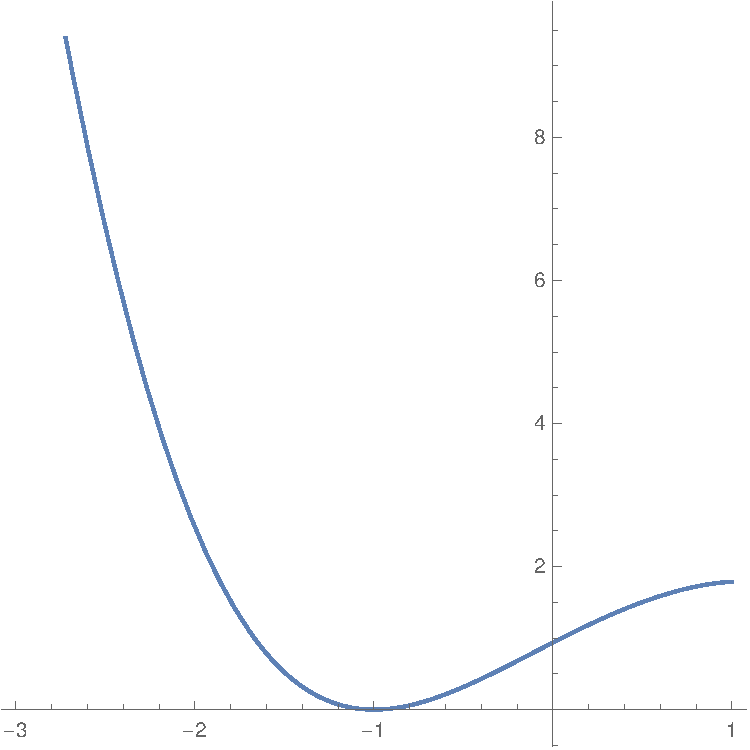
\includegraphics[width=\textwidth]{A8p6.pdf}
		\else
			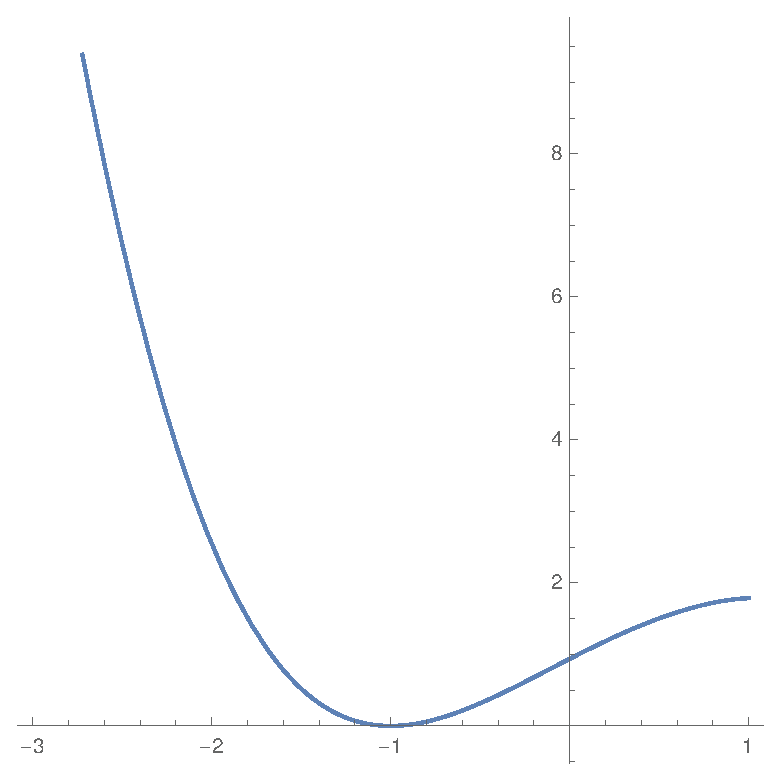
\includegraphics[width=\textwidth]{A8p6.eps}
		\fi
		\caption{Plot of \(g(y) = \min_{x} f(x, y)\)}
		\label{mathematica}
	\end{figure}
\end{proof}


\section{Application}
The length, \(L\), of the longest ladder that can pass around the corner of two corridors depends on the angle \(\alpha\) shown in Figure \ref{ladder}.
\ifnum\webview=1
	\begin{figure}[H]
\else
	\begin{figure}[htbp]
\fi
	\centering
		\ifpdf
			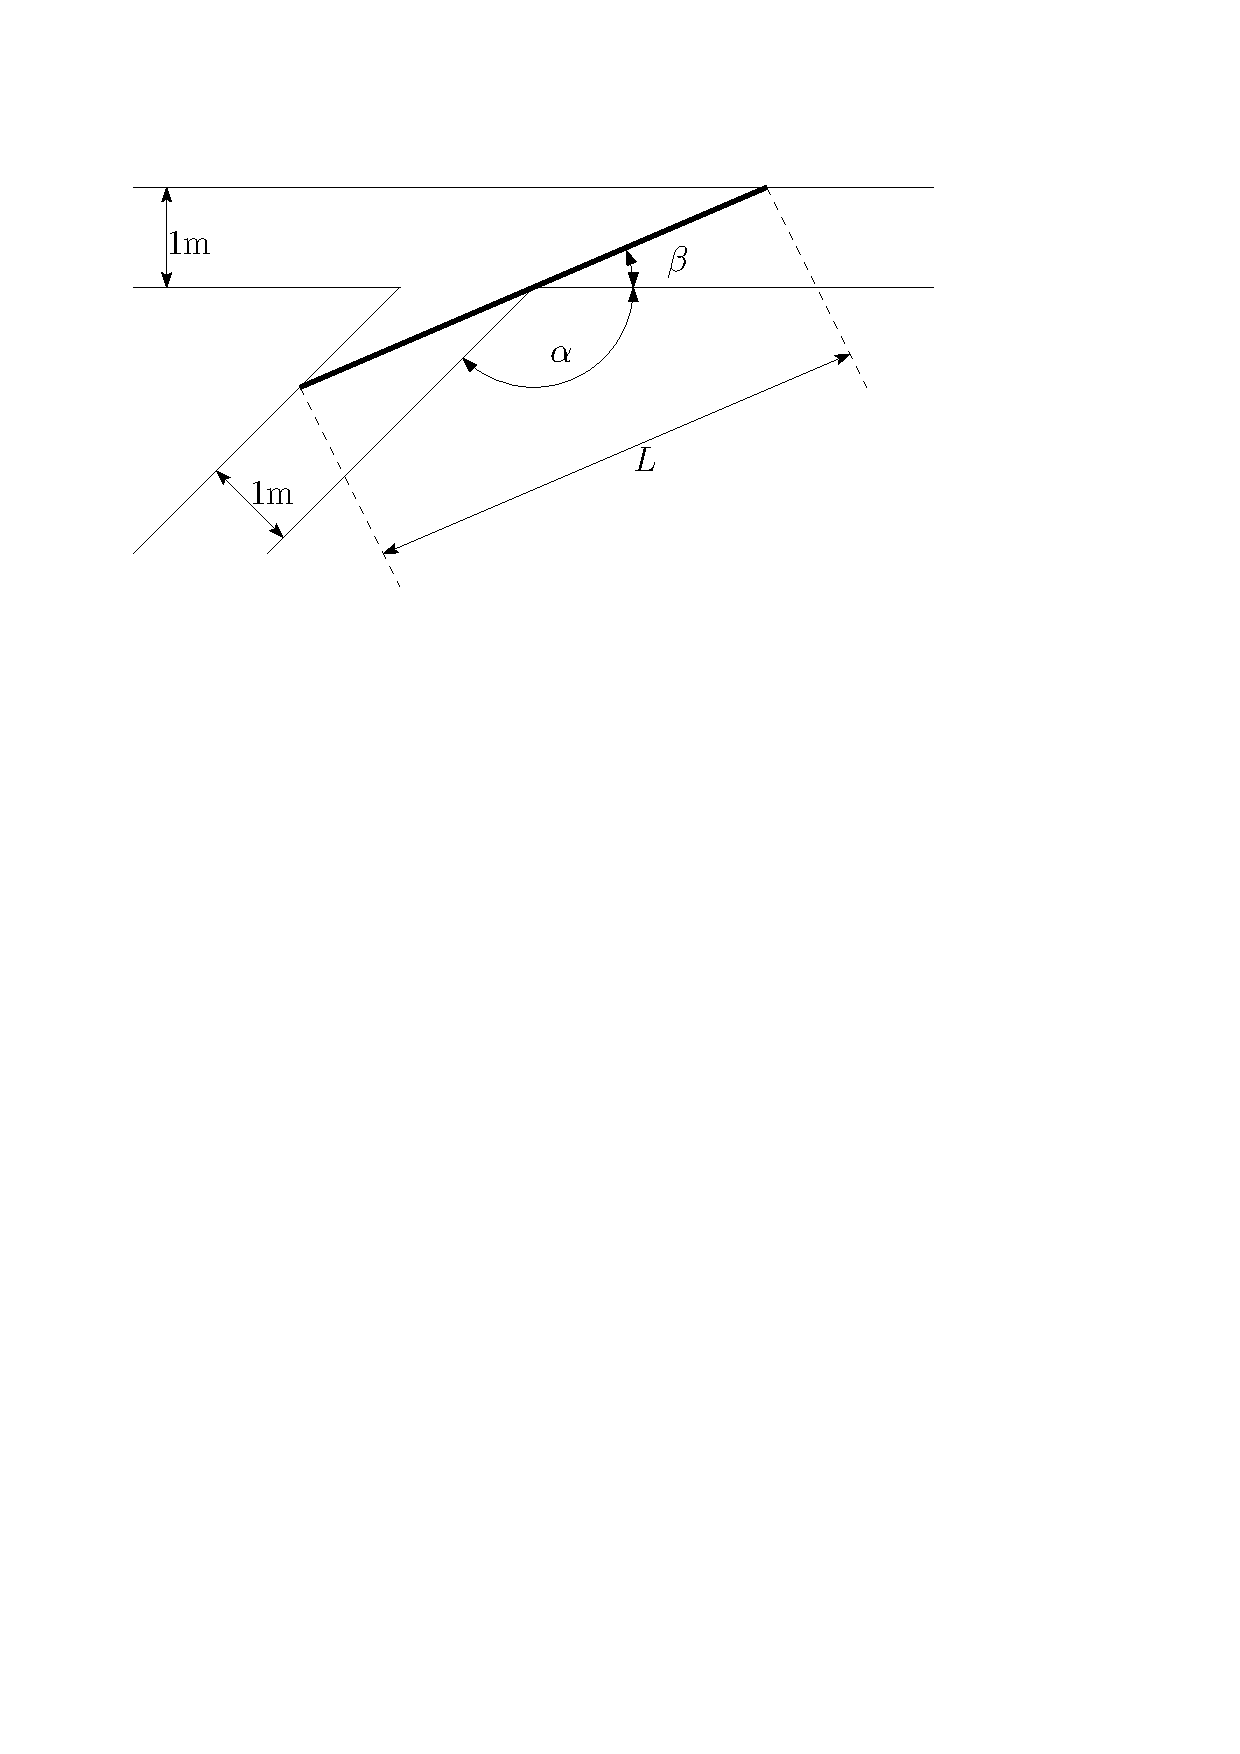
\includegraphics[width=\textwidth]{A8p7.pdf}
		\else
			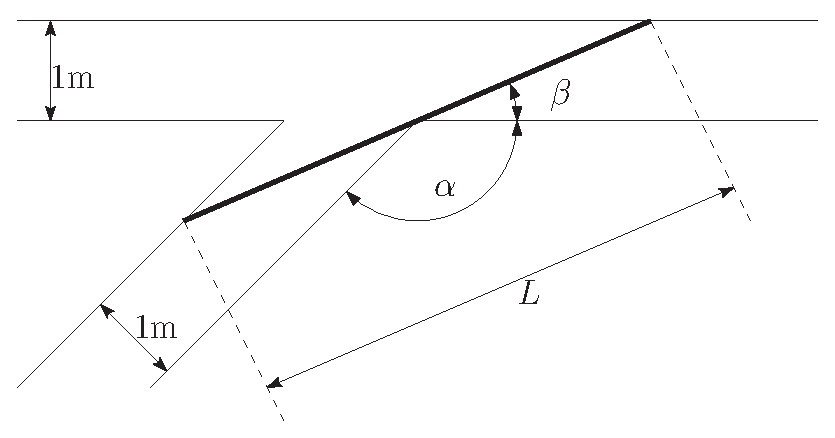
\includegraphics[width=\textwidth]{A8p7.eps}
		\fi
		\caption{Illustration of the situation}
		\label{ladder}
	\end{figure}
Produce a MATLAB\texttrademark\ plot of \(L\) versus \(\alpha\) ranging from \(45^\circ\) to \(135^\circ\) by first solving a minimisation problem using numerical methods that we have discussed so far.
\begin{proof}[Answer]
Observe that
\[ L(\alpha,\beta)=\frac{1}{\sin\beta}+\frac{1}{\sin(\alpha+\beta)}. \]
Regard \(\alpha\) as a parameter, and \(\beta\) as a variable, we need to find
\[ l(\alpha)=\min_{\beta}L(\alpha,\beta). \]
So we require
\[ \partial_\beta L(\alpha,\beta)=0, \quad \partial_{\beta\beta} L(\alpha,\beta)>0. \]
Plug in the function, we find that when
\[ \beta=\frac{\pi-\alpha}{2}, \]
the condition is satisfied.
Thus,
\[ l(\alpha)=L\left(\alpha,\frac{\pi-\alpha}{2}\right)=\frac{1}{\sin\frac{\pi-\alpha}{2}}+\frac{1}{\sin\frac{\pi+\alpha}{2}}. \]
The graph of this function on the desired domain is plotted in Figure \ref{laddersolution}.
\ifnum\webview=1
	\begin{figure}[H]
\else
	\begin{figure}[htbp]
\fi
	\centering
		\ifpdf
			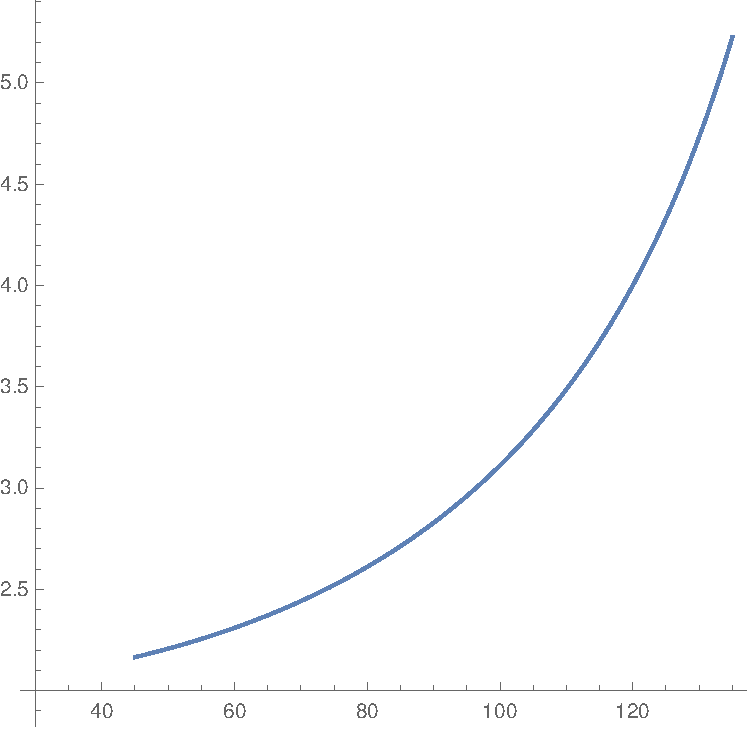
\includegraphics[width=\textwidth]{A8p7s.pdf}
		\else
			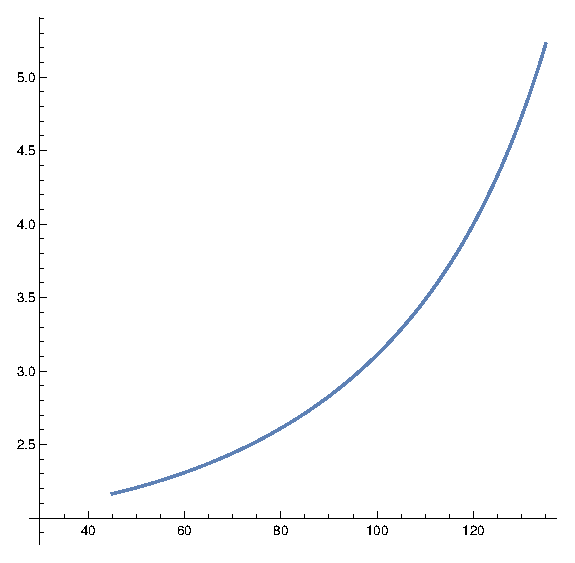
\includegraphics[width=\textwidth]{A8p7s.eps}
		\fi
		\caption{Maximum length to pass the corridors. (\(\beta\) in degrees)}
		\label{laddersolution}
	\end{figure}
\end{proof}


\section{Method of simulated annealing}
A popular global optimization algorithm for difficult functions, especially if there are many local minima, is called the \emph{method of simulated annealing}.
It involves no derivatives or an initial guess that needs to be sufficiently close to the minimum.
Suppose \(f:\R^n \to \R\) has a global minimum at \(x^∗\) and the $k$-iteration \(x_k\) has been computed.
It iterates by the following scheme:
\begin{enumerate}
	\item Generating a number of random points \(u_1, u_2,\cdots, u_m\) in a large neighborhood of \(x_k\).
	\item Computing \(f(u_1), f(u_2),\cdots, f(u_m)\).
	\item Finding the index \(j\) such that \(f(u_j)=\min\{f(u_1), f(u_2),\cdots, f(u_m)\}\).
	\item Assigning \(x_{k+1}=u_j\) if \(f(x_k)>f(u_j)\).
	Otherwise assigning a probability
	\[ p_i=\frac{\exp\{\alpha[f(x_k)-f(u_i)]\}}{\sum_{\ell=1}^{m}\exp\{\alpha[f(x_k)-f(u_\ell)]\}}, \quad \alpha>0, \]
	to \(u_i\) for each \(i=1, \cdots, m\).
	Then making a random choice among \(u_1, u_2,\cdots, u_m\) according to the probabilities \(p_i\) and assigning this randomly chosen \(u_\ell\) to be \(x_{k+1}\).
\end{enumerate}
With some minor modifications, this can be used for function \(Q: \mathcal{X}\to\R\), where \(\mathcal{X}\) is any set.
For example, in the \emph{traveling salesman problem}, \(\mathcal{X}\) is the set of all permutations of a set of integers.
Consider the \emph{Euclidean traveling salesman problem} (ETSP):
given a set of points in \(\R^2\) representing positions of cities on a map, we wish to visit each city exactly once while minimizing the total distance traveled.
\begin{enumerate}
	\item Implement simulated annealing to solve ETSP with different \(\alpha\).
	\item Propose another optimization method to solve ETSP.
	Analyze how its efficiency would compare to that of simulated annealing.
\end{enumerate}